
%(BEGIN_QUESTION)
% Copyright 2009, Tony R. Kuphaldt, released under the Creative Commons Attribution License (v 1.0)
% This means you may do almost anything with this work of mine, so long as you give me proper credit

Determine the amount of differential pressure ``seen'' by the DP transmitter based on the two pressure gauges' readings and the valve statuses, being sure to note whether this pressure will be interpreted by the DP transmitter as a {\it positive} or a {\it negative} value:

$$\includegraphics[width=15.5cm]{i03725x01.eps}$$

\underbar{file i03725}
%(END_QUESTION)





%(BEGIN_ANSWER)

$\Delta P$ = 0 PSI

%(END_ANSWER)





%(BEGIN_NOTES)

{\bf This question is intended for exams only and not worksheets!}.

%(END_NOTES)


